

%%%%%%%%%%%%%%%%%%%%%%%%%%%%%%%%%%%55%%
\begin{frame} [plain]
    \frametitle{}
    \Background[1] 
    \begin{center}
    {\huge 第3讲:量子信息处理-逻辑门}
    \end{center}  
    \addtocounter{framenumber}{-1}   
\end{frame}
%%%%%%%%%%%%%%%%%%%%%%%%%%%%%%%%%%

\section{1.逻辑门的可逆性}

\begin{frame} 
    \frametitle{经典加法器}
    \begin{tcolorbox2}{信息学基本原理}
    所有类型的计算都是加法,二进制加法是逻辑运算,逻辑门是实现各种逻辑运算的基础性元件。
    \end{tcolorbox2}
    \例[1. 设计一个加法器,实现两整数之间的求和]{}
    \解~对于小于$2^n$的正整数$M,N$可表示为:
    \[M=\sum_{i=0} ^{n-1} a_i 2^i,\qquad N=\sum_{i=0} ^{n-1} b_i 2^i\]
\end{frame} 

\begin{frame}    
    \begin{table}
        \caption{加法器真值表,其中 $s_i, c_{i+1}$分别是求和位和进位}
        \begin{tabular}{@{} llll @{}}
          %\toprule
          $a_i$ & $b_i$ & $s_i$ & $c_{i+1}$\\
          \midrule
          0 & 0 & 0 & 0 \\
          0 & 1 & 1 & 0\\
          1 & 0 & 1 & 0\\
          1 & 1 & 0 & 1\\
          \bottomrule
        \end{tabular}
      \end{table}
    \begin{itemize}
        \IItem $a_i$, $b_i$ 不同时, $s_i$置“1”,否则置“0” : 逻辑“异或” XOR  $\qquad s_i=a_i\oplus b_i $
        \IItem $a_i$, $b_i$ 都是1时, $c_{i+1}$置“1”,否则置“0”:   逻辑“与” AND  $\quad c_{i+1}=a_i \wedge b_i $
    \end{itemize}
\end{frame} 

\begin{frame} 
    \frametitle{}
\centering
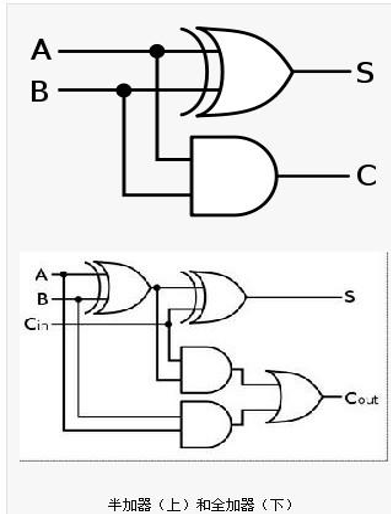
\includegraphics[width=0.45\textwidth]{figs/10.png}
\end{frame} 

\begin{frame} {可逆性}
    考察发现:经典 XOR 门和 AND 门都是不可逆的!\\
    不可逆过程有深刻的物理内含:
    \begin{itemize}
        \IItem 不可逆过程熵增加 $S=k_B\ln\Omega$
        \IItem 不可逆过程信息丢失 $\Delta S=k_B\ln2 $
        \IItem 不可逆过程消耗能量
        \IItem 不可逆过程不是幺正变换
    \end{itemize}
    当前通用的图灵机都是不可逆的! \\ \vspace{0.8em}
    {\Bullet}~~量子计算机通过酉操作(幺正变换)来实现信息处理,要求所有的逻辑门都是可逆的!\\
    
\end{frame}  

\begin{frame} 
    \begin{tcolorbox2}{Bennett 证明}
    所有不可逆的计算机都可以改造为可逆计算机
    \end{tcolorbox2}
    \例[2. 试把不可逆的异或门,改造为可逆的异或门]{}
    \解~改造方法如图 \\
    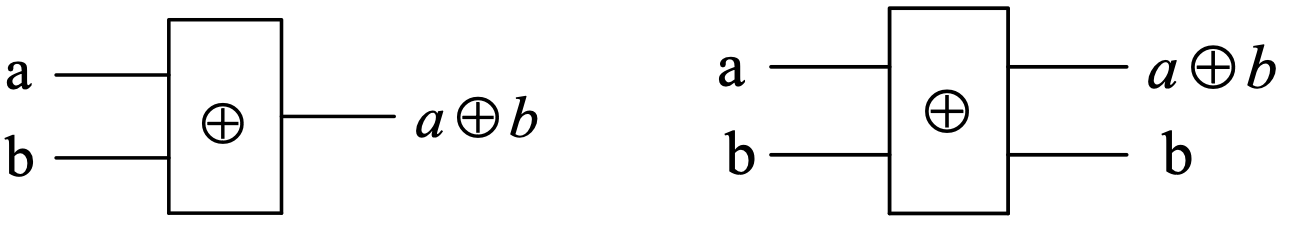
\includegraphics[width=0.7\textwidth]{figs/11.png}
    
    可逆源于所有信息被保留,信息的擦除消耗能量增加熵,导致不可逆。
\end{frame} 



\begin{frame}{}
        \frametitle{麦克斯韦妖佯谬-1871}
        绝热容器分成两格,中间是由“妖”控制的一扇“门”,分子作无规则热运动时会向门上撞击,“门”可以选择性的将速度较快的分子放入一格,
        较慢的分子放入另一格. 这样,体系的熵在减少!\\
       \begin{center}
        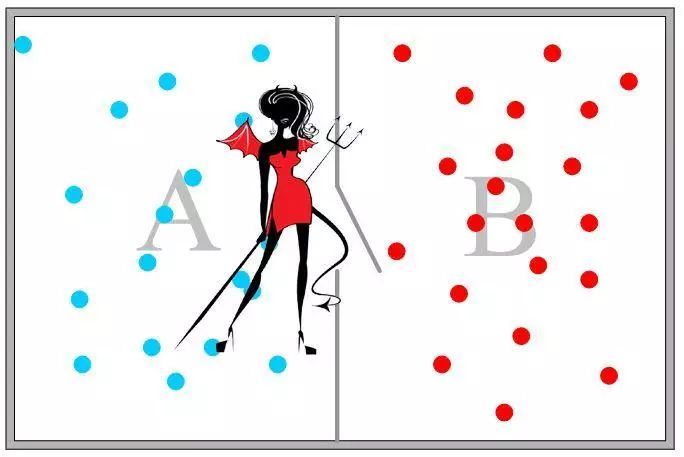
\includegraphics[width=0.42\textwidth]{figs/12.png}     
       \end{center}   
       1981年,Bennett证明“妖”必须去除前面分子的信息,这消耗能量并导致$k_B\ln2$的熵增。 
\end{frame} 

\begin{frame}
    基本结论:\\
   \begin{itemize}
       \IItem 微观过程是可逆的
       \IItem 微观过程服从量子力学原理
       \IItem 演化过程是幺正的
       \IItem 基于幺正变设计的量子逻辑门是可逆的
       \IItem 如果有一套普适的量子逻辑门,发展量子计算机是可行的
   \end{itemize} 
\end{frame} 

\section{2.单量子比特逻辑门}

\begin{frame}
    \frametitle{单量子比特逻辑门}   
单量子比特波函数:
\[\rs{\psi} =\alpha\rs{0}+\beta\rs{1}, \qquad (|\alpha|^2+|\beta|^2=1)\]
矩阵:
 \[ \rs{\psi}=\begin{bmatrix}
    \alpha \\
    \beta
 \end{bmatrix}\]
 因此,单比特逻辑门是操作$C^2$空间的$2\times 2$的矩阵,\\
 由于可逆性的要求,单比特逻辑门也必须是幺正(酉)矩阵。 
\end{frame} 

\begin{frame} 
    \frametitle{1. 量子非门(X-Gate)} 
    经典非门: $0\to 1, \qquad 1 \to 0$ \\
    量子非门: $\alpha\rs{0}+\beta\rs{1} \quad \to \quad\alpha\rs{1}+\beta\rs{0}$ \\ \vspace{1em}

    \例[2. 试证明$\sigma_x$矩阵就是单比特量子非门]
    {~~\\
    \[X \equiv \sigma_x=\XGate = \lr{0}{1}+\lr{1}{0}\]} 
    \证~(1)对于$\rs{\psi} =\alpha\rs{0}+\beta\rs{1}$,有
    \[X \rs{\psi} = X \Qbit{\alpha}{\beta}=\XGate\Qbit{\alpha}{\beta} =\Qbit{\beta}{\alpha}=\beta\rs{0}+\alpha\rs{1}=\alpha\rs{1}+\beta\rs{0}
    \]
\end{frame} 

\begin{frame}     

    (2)幺正性
    \[X^\dagger =(X_{ij} ^*)^T=\XGate\]
    \[X^\dagger X = XX^\dagger =\XGate \XGate=I\]
    证毕!\\ \vspace{1em}
    {\Bullet} 很明显,这是比特反转
    \[ X\rs{0}= \rs{1},\qquad X\rs{1}= \rs{0}
    \]

\end{frame}

\begin{frame}{2.基矢变换门(H-Gate)}
    基矢变换: $\rs{0} \to \rs{+}, \qquad \rs{1} \to \rs{-} $
    \例[4. 试证明如下矩阵就是基矢变换门]
    {~~\\
    \[H \equiv \frac{1}{\sqrt{2}}(X+Z) =\HGate \]} 
    \证~(1)
    \[H \rs{0}= \HGate\Qbit{1}{0}=\frac{1}{\sqrt{2}}\Qbit{1}{1} = \frac{1}{\sqrt{2}}\Qbit{1}{0} +\frac{1}{\sqrt{2}}\Qbit{0}{1} =\frac{\rs{0}+\rs{1}}{\sqrt{2}} =\rs{+}\]
    \[\text{同理}\qquad H \rs{1}=\frac{\rs{0}-\rs{1}}{\sqrt{2}} =\rs{-}\]
\end{frame}

\begin{frame}{}
    (2)幺正性
    \[H^\dagger H = HH^\dagger=I\]
    证毕! \\ \vspace{0.6em}
    \[H \rs{0}=\frac{\rs{0}+\rs{1}}{\sqrt{2}}\]
    \[H \rs{1}=\frac{\rs{0}-\rs{1}}{\sqrt{2}}\]
    {\Bullet} 统一表示为:(x,z 分别取0或1)\\
    \[H \rs{x}=\frac{\sum_z(-1)^{xz}\rs{z}}{\sqrt{2}}\]
\end{frame}

\begin{frame}
    \frametitle{}
    {\Bullet} 可以证明~H 也是自共轭矩阵,有: \[H^\dagger =H \to H^2=I\]
    \例[5. 试证明H可以完成反向变换]
    {~~\\
    \[H \rs{+}= \rs{0}, \qquad H \rs{-}= \rs{1}  \]} 
    \证~ \[H\rs{0}=\rs{+}, \qquad H \rs{0}= \rs{-} \]
    \[HH\rs{0}=H\rs{+} , \qquad H H\rs{0}= H\rs{-}\]
    \[\rs{0}=H\rs{+} , \qquad \rs{0}= H\rs{-}\]
    证毕!
\end{frame}

\begin{frame}
    \frametitle{3. 相位反转门(Z-Gate)} 
    相位反转: $\alpha\rs{0}+\beta\rs{1} \quad \to \quad\alpha\rs{0}-\beta\rs{1}$ \\ \vspace{0.6em}
    \例[3. 试证明$\sigma_z$矩阵就是相位反转门]
    {~~\\
    \[Z \equiv \sigma_z =\ZGate =-i\lr{0}{1}+i\lr{1}{0}\]} 
    \证~(1)
    \[Z \Qbit{\alpha}{\beta}=\ZGate\Qbit{\alpha}{\beta} =\Qbit{\alpha}{-\beta}\]
    (2)幺正性
    \[Z^\dagger Z = ZZ^\dagger=I\]
    证毕!~~ {\Bullet} 很明显~~$ Z\rs{0}=\rs{0},\quad Z\rs{1}=-\rs{1}= e^{i\pi}\rs{1}$
\end{frame}

\begin{frame}
    \frametitle{4. 各种相位门} 
    既然态矢都在 Block球面,那相位反转(Z-Gate)就是绕Z轴旋转180度($\pi$),当然有绕Z轴旋转90度($\dfrac{\pi}{2}$)的门,这就是S-Gate.\\
    \[Z\rs{1}= e^{i\pi}\rs{1}\]
    \[S\rs{1}= e^{i\pi/2}\rs{1}\]
    由此得:\\
    \[S \equiv \SGate = {\begin{bmatrix}
        1 & 0 \\
        0 & e^{\frac{i\pi}{2}}
     \end{bmatrix}}\]
    所以S-Gate=$\sqrt{Z}$-Gate 
\end{frame}
    
\begin{frame}
    当然,也有绕Z轴旋转45度的门,称为T-Gate,也称 $\pi/8$-Gate
    \[S \equiv \SGate = {\begin{bmatrix}
        1 & 0 \\
        0 & e^{\frac{i\pi}{4}}
     \end{bmatrix}}\]
    绕Z轴旋转任意角度($\phi$)的门,则称为旋转门$R_\phi$-Gate
    \[R_\phi \equiv  \RGate \]
    {\Bullet} 很明显~~$ R_\phi\rs{0}=\rs{0},\quad R_\phi\rs{1}= e^{i\phi}\rs{1}$
\end{frame}

\section{3.双量子比特逻辑门}

\section{4.多量子比特逻辑门}

\section{5.普适逻辑门}

\begin{frame}
    \frametitle{}
    \begin{tcolorbox3}[学术讨论]
        基于以上4个假定,可以从数学上在Hilbert空间导出整个量子力学体系,那么基于假定导出的量子力学可靠吗?
    \end{tcolorbox3}
\end{frame}